\documentclass[border=2mm]{standalone}
\usepackage{tikz,pgfplots}
\pgfplotsset{compat=1.14}
\usetikzlibrary {datavisualization.polar}

\begin{document}
\begin{tabular}{c}
\begin{tikzpicture}[scale=0.9]
\begin{axis}[
	%scatter/classes={i={mark=o,draw=black}},
	ticks=none,
    axis lines = middle,
    axis line style={->},
    ymin=-0.025,ymax=1,
    xmin=-0.2, xmax=1,
    axis equal image]
%\addplot[scatter,only marks,scatter src=explicit symbolic] 
\addplot+ [nodes near coords,only marks,mark size=1.5pt,purple,
       point meta=explicit symbolic]
table[meta=label] {
     x      y       label
0.886327   0.156283 $z_0$
0.761151   0.277036 $z_1$
0.502602   0.421733 $z_2$
0.07475    0.423927 $z_3$
-0.174127  0.063377 $z_4$
%0.026304  -0.022071 $z_5$
0.000205  -0.001161 $z_6$
    };
\draw (axis cs:0,0) circle [radius=1];  
\end{axis}
\end{tikzpicture}

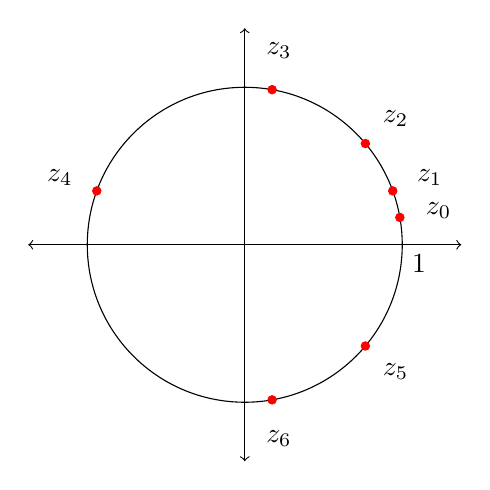
\begin{tikzpicture}
\draw[thin] (0cm,0cm) circle(2cm);
\draw[<->] (-2.75,0) -- (2.75,0);
\draw[<->] (0,-2.75) -- (0,2.75);
\foreach \x in {10, 20, 40, 80, 160, 320, 640} {
               \filldraw[red] (\x:2cm) circle(1.5pt);
               }
\foreach \x/\xtext in {
            10/z_0,
            20/z_1,
            40/z_2,
            80/z_3,
            160/z_4,
            320/z_5,
            640/z_6
           }
            \draw (\x:2.5cm) node[fill=white] {$\xtext$};
\node[below right]  (c) at (2,0) {1};
\end{tikzpicture}
\\
\begin{tikzpicture}
\begin{axis}[
	ticks=none,
    axis lines = center,
    axis line style={<->},
    ymin=-9,ymax=3,
    xmin=-6, xmax=1.5,
    axis equal image]
\addplot+ [nodes near coords,only marks,mark size=1pt,purple,
       point meta=explicit symbolic]
table[meta=label] {
    x        y        label 
 0.930977    0.5375   $z_0$
 0.577813    1.000801 $z_1$
-0.667735    1.15655  $z_2$
-0.891739   -1.544537 $z_3$
-1.590397    2.754648 $z_4$
-5.058723   -8.761964 $z_5$
    };
\draw (axis cs:0,0) circle [blue, radius=1];  
\end{axis}
\end{tikzpicture}
\end{tabular}
\end{document}
     